\chapter{多摄像头系统的拍摄时间检测}

\section{本章引言}

对于多摄像头系统来说,控制各个摄像头在特定时刻进行拍摄是其主要的同步方法。在实际的系统应用过程当中,服务器会通过网络发送信号,控制各个摄像头进行拍摄,但是在系统内可能存在多种因素导致摄像头的真实拍摄时间与服务器设定的拍摄时间不符,而这也就导致了多摄像头系统内存在的同步误差。比如服务器发送命令控制各个摄像头在$t_1$时间后进行拍摄,但是服务器程序运行会消耗一定的时间$t_2$,控制命令经网络由服务器传输给各个摄像头,传输过程会消耗一定时间$t_3$。摄像头接收到命令设定自身参数在$t_1$时间后拍摄,而在$t_1$时刻摄像头开始拍摄时,又会消耗掉一定的硬件响应时间$t_4$,因此摄像头真实的拍摄时间并非服务器设定的$t_1$,而是$T = t_2 + t_3 + t_1 + t_4$。并且系统中可能存在的各种延时随机出现,对于各个摄像头来说其延时长短也同样不确定,无法准确进行预测。

\begin{figure}[h] 
  \centering
  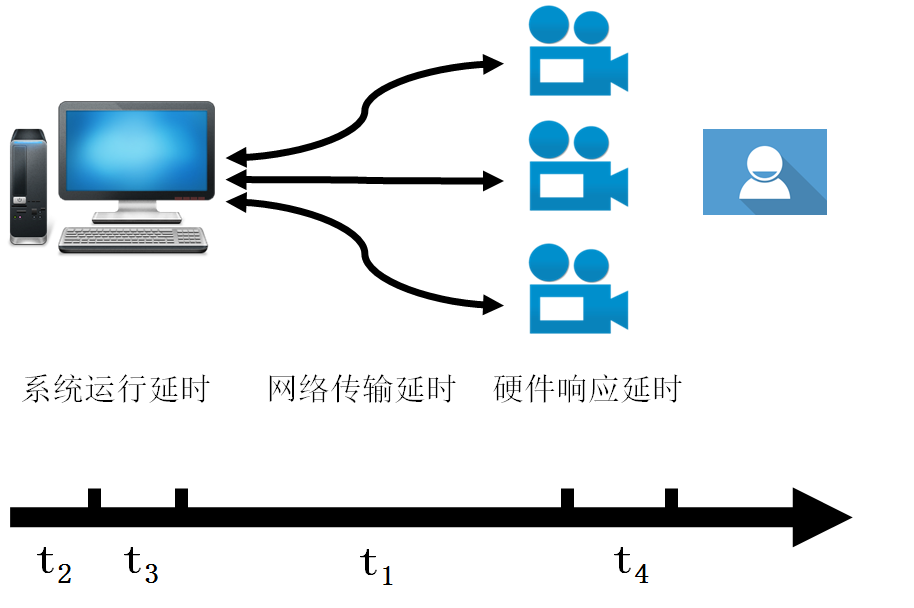
\includegraphics[height=6.5cm, width=8.5cm]{延时}
  \caption{多摄像头系统拍摄过程中可能存在延时}
\end{figure}

因此,对于多摄像头系统来说,为了提高同步精度,并且检验同步效果,就不能仅仅依靠系统内部时钟虽显示的时间进行判断,需要借助外界参考物来检测各个摄像头的拍摄时间。本章提出了一种基于LED点阵的拍摄时间检测方法。该方法利用FPGA控制LED点阵作为检测器,通过设计不同编码方法使点阵显示不同的状态序列。当摄像头拍摄到检测器图像后,对图像进行分析,从而检测出摄像头真实的拍摄时间。该方法通过图像进行检测,排除了系统内部各项误差因素的干扰,并且检测器与摄像头相互分离无需数据通信,同时还适用于多种帧率、曝光时间的摄像头,保证了该方法的普适性。通过对检测器参数的调整可以实现不同精度的检测,且无需调整摄像头参数,使得该方法能够在摄像头正常工作过程中实时进行检测。

\section{拍摄时间检测方法}

采用本方法对摄像头拍摄时间进行检测,主要可分为如下3个步骤:

\textbf{(1)检测器初始化:}该方法的检测器由FPGA控制器和LED点阵两部分组成,分别实现了系统控制和检测信号显示的功能。在初始化阶段,编写控制程序利用FPGA控制LED点阵中各个LED灯的亮灭变化,显示出不同的LED灯组合状态。当每个状态持续一段时间,若干不同状态即可组成状态序列。因此,通过调整FPGA的控制策略,即可控制LED点阵服从一定的编码规律。而根据此规律又可以确定每个LED点阵状态在状态序列当中所处的位置,即可确定每个状态出现的时间。

\textbf{(2)获取检测图像:}设置好检测器后,在需要对拍摄时间进行检测时,将LED点阵置于多摄像头系统的拍摄范围内,控制各个摄像头对其进行拍摄,并将图像保存供分析处理,只需保证拍摄到的图像清晰、完整即可。由于检测器独立于多摄像头系统,相互之间无需进行通信,避免了信号连接、传输、识别等众多操作,有效扩大了该检测方法的适用范围。

\textbf{(3)分析图像计算拍摄时间:}当获得各个摄像头拍摄到的LED点阵图像后,利用图像处理服务器对各副图像进行处理分析。在每幅图像当中提取LED点阵所在位置,并分析点阵当中各个LED灯的亮灭情况,即LED点阵在摄像头拍摄时刻的状态,从而可以根据LED点阵的编码规律确定此状态在序列当中所处的位置,即可以推断摄像头拍摄的时间。多个摄像头之间也可以根据拍摄到的状态的不同确定拍摄时间间隔。

根据在初始化时选择的编码方式的不同,检测出的拍摄时间精度也不尽相同。为了提高该方法的检测精度,要求每个LED点阵状态的持续时间较短,因此要求LED点阵的变化频率较高,对于控制信号的响应速度较快。同时,为了使状态序列足够长,要求LED点阵包含足够多的LED灯,使其能够组合成足够多的不同状态。另外,由FPGA控制LED点阵中各个LED灯期进行变化,因此要求FPGA具有特定接口能够向LED点阵发送控制信号。并且为了在点阵高频率变化时保证足够的时间精度,要求FPGA处理信号和传输信号的时间延迟要尽可能小。对于图像识别服务器来说,为了保证检测的准确性和高精度要求,其对于LED点阵的识别和对于LED灯亮灭状态的判断需要具有更高的准确性。

\section{LED点阵编码方法}
\label{codeMe}

对LED点阵中各个LED灯的亮灭变化情况进行编码,目的是为了使每个由LED灯组成的点阵状态具有唯一性,并且形成特定的状态序列,以便能够对摄像头拍到的状态进行识别,确定该状态在序列中所处的位置,同时还要尽可能提高识别正确率。因此,对于点阵编码方法,要求其具有唯一性、有序性、易识别性。针对以上要求,本文提出了以下4种编码方法,并对其进行了比较。不失一般性,以下采用如图~\ref{mat} 所示的4 × 4的LED点阵对编码方法进行描述。

\begin{figure}[h] 
  \centering
  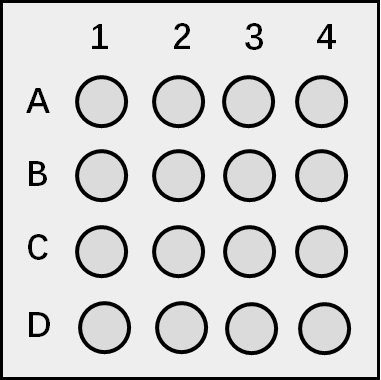
\includegraphics[height=4cm, width=4cm]{点阵}
  \caption{4 × 4的LED点阵}
  \label{mat}
\end{figure}

该点阵共有16个LED灯,依次编号A1、A2、...、B1、B2、...、D4。各个LED灯的亮灭状态相互独立。各个LED灯周期性变化,每个控制周期的持续时间($t_{dur}$)相同。每一个控制周期内,各个LED灯保持亮灭不变,全部LED灯的亮灭状态组成LED点阵在该周期内的状态,全部LED点阵状态组成该编码方法生成的状态序列。各LED灯的亮灭状态和控制周期的时间长短由FPGA控制器进行控制,且控制周期持续时间远远大于LED灯亮灭响应时间和控制信号生成、传输时间。

\subsection{流水编码}
\label{flow1}

流水编码方法控制LED点阵在一个控制周期内仅有一个LED灯点亮,下一个周期时下一个LED灯点亮,上一周期点亮的LED灯熄灭。各LED灯按照由左至右、由上至下的顺序依次点亮。当最后一个LED灯,即D4灯点亮后,下一周期时D4灯熄灭、A1灯点亮,进行下一循环,如图~\ref{flow}所示:

\begin{figure}[h] 
  \centering
  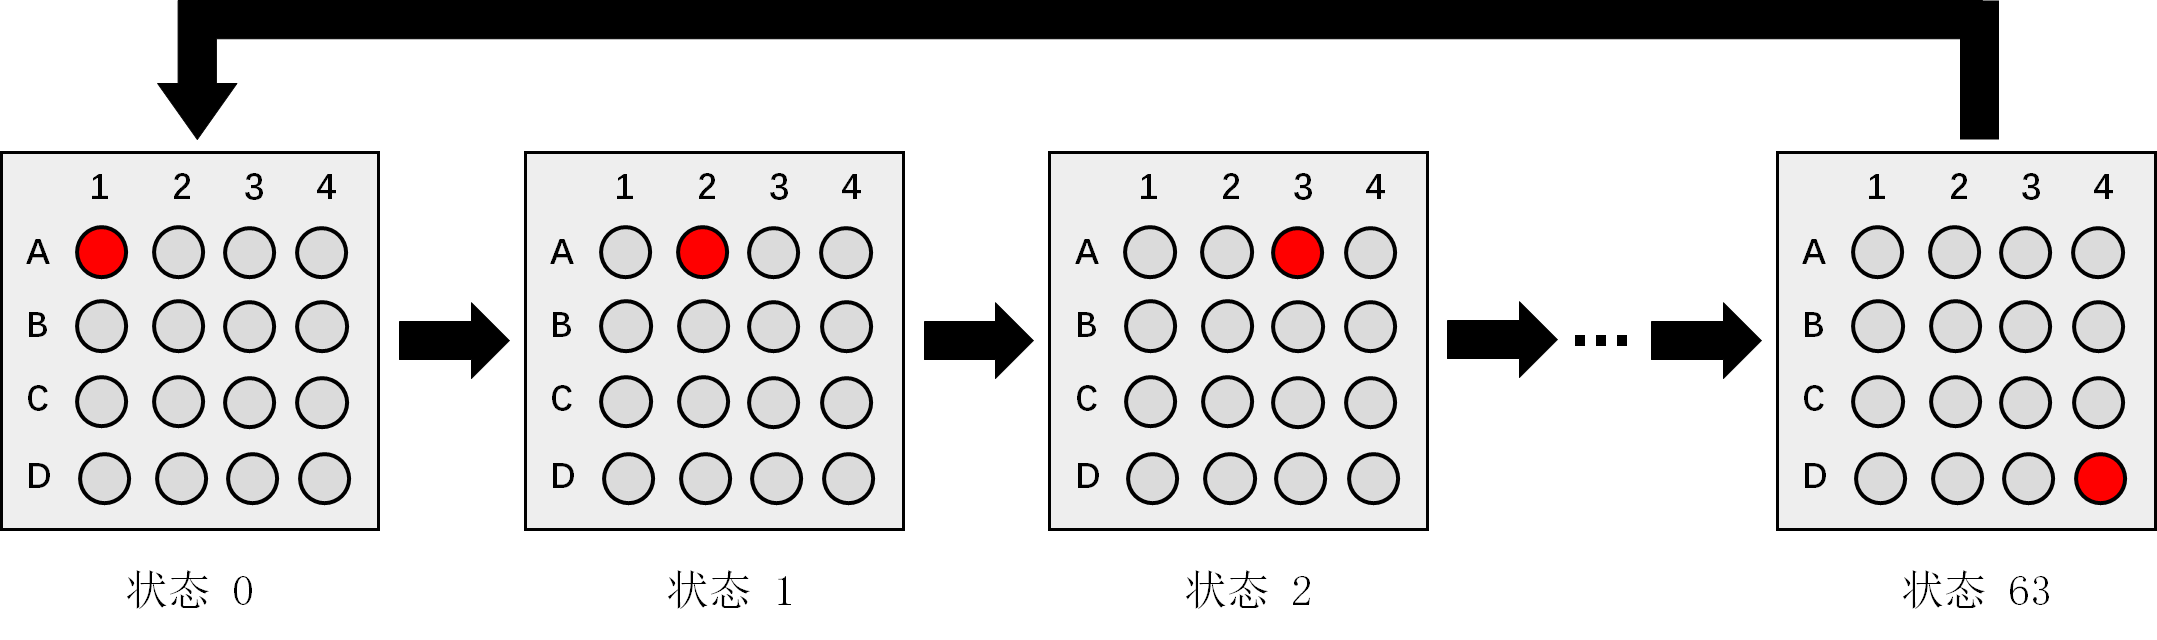
\includegraphics[height=3.6cm, width=12cm]{flow}
  \caption{流水编码的点阵状态序列}
  \label{flow}
\end{figure}

该编码方法实现较为简单,当LED点阵共包含$n$个LED灯,控制周期时间长度为$t_{dur}$时,从第一个LED灯点亮到最后一个LED灯点亮,即一个总的循环周期时间长度($T$)为:

\begin{equation}
T = n * t_{dur}
  \label{flowE}
\end{equation}

当摄像头拍摄到第$k$个状态时,即可以判定其拍摄时刻与LED点阵开始运行时刻之间的时间差为 $k * t_{dur}$。对于两个摄像头分别拍摄到第$k_1$和$k_2$个状态,则这两个摄像头之间的时间差为$(k_1 - k_2) * t_{dur}$。

当摄像头拍摄到某一LED点阵的状态时,可能是在LED点阵保持状态不变的整个控制周期$t_{dur}$中的任意时刻进行拍摄的,因此其检测精度与控制周期的大小有关,最大误差为控制周期时间长度。因此,为了提高检测精度,往往需要控制周期$t_{dur}$较小。同时当LED灯数量较少时,根据公式~\ref{flowE}可知,该编码算法的总循环周期$T$较短。这可能导致在测量过程中使用摄像头拍摄到的不同状态处于不同循环周期内,且无法确定其所属的循环周期,因此最终的测量结果为$x * T + k * t_{dur}$,其中$x$可以取$0, 1, 2...$,总循环周期过小会导致无法确定$x$取值,使得测量结果存在误差。

\subsection{二进制编码}

此编码方法中,将每一个LED灯视为一个二进制数位,LED灯点亮代表1、熄灭代表0,整个LED点阵视为一个16位的二进制数。在每个控制周期内,LED点阵显示一个二进制数,下一个周期时发生变化,按照二进制数变化规律显示下一个二进制数。状态序列如图~\ref{binary}所示:

\begin{figure}[h] 
  \centering
  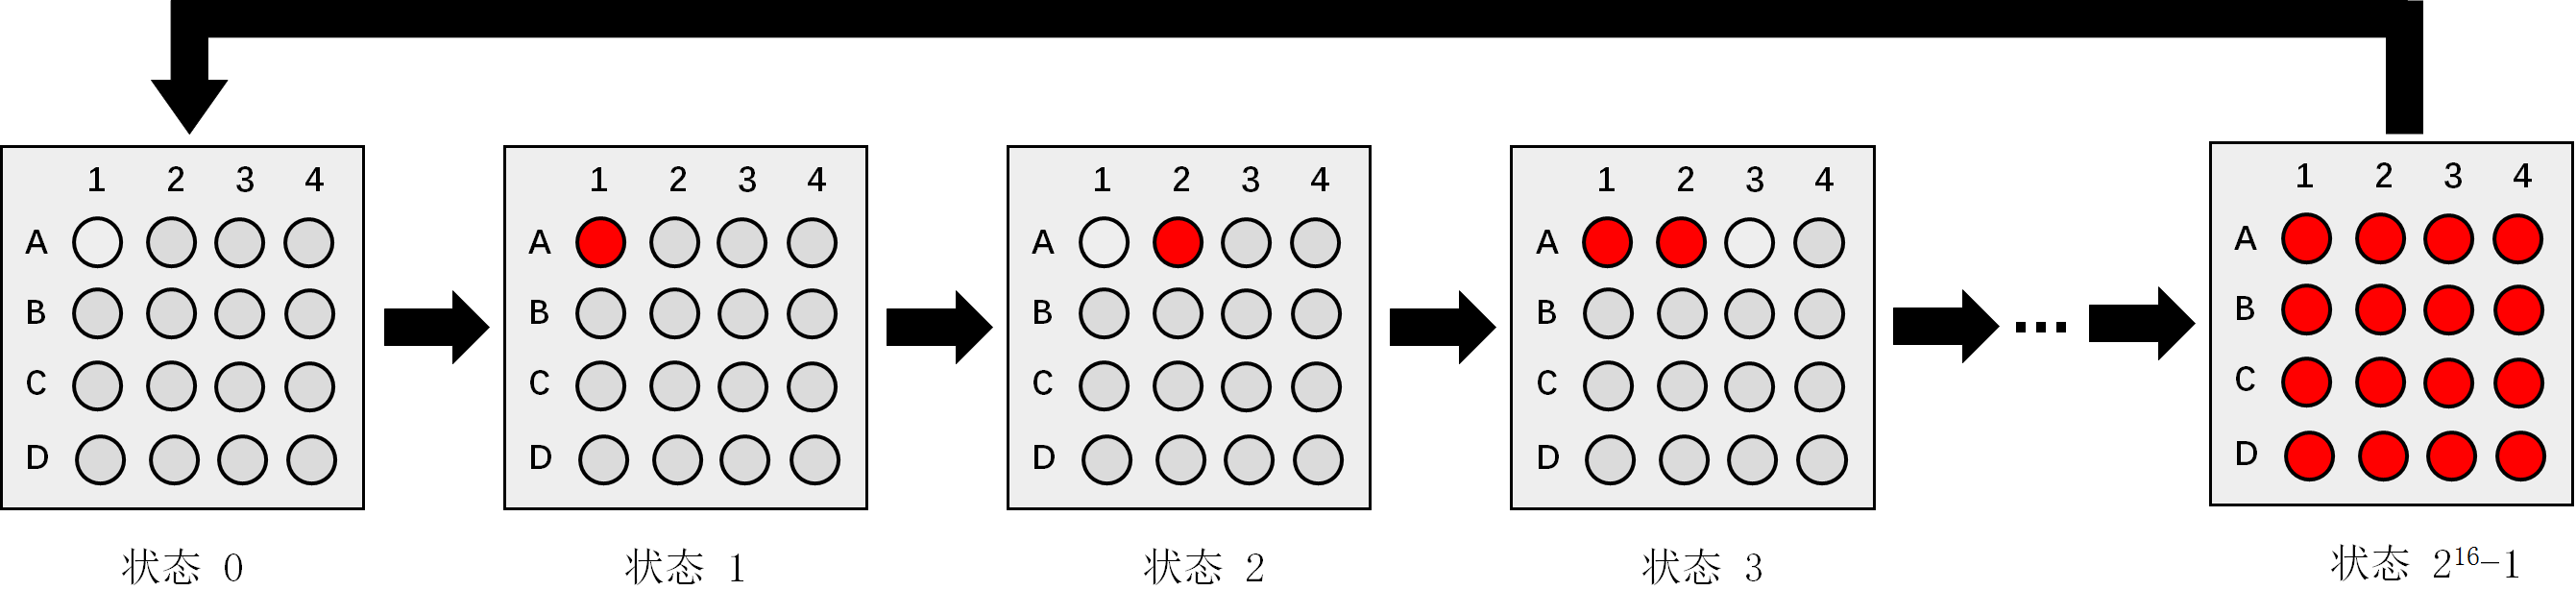
\includegraphics[height=3.6cm, width=14cm]{binary}
  \caption{二进制编码的点阵状态序列}
  \label{binary}
\end{figure}

使用该编码方法,当LED点阵共包含$n$个LED灯时,一个总的循环周期内共有$2^n$个LED点阵状态,则一个总的循环周期的时间长度为:

\begin{equation}
T = 2^n * t_{dur}
\end{equation}

循环周期的时间长度随着LED灯的数量指数增长,因此可以利用较少的LED灯实现较长的循环周期,使得在检测过程中不会出现不同状态属于不同循环周期的情况。二进制编码方法的检测精度同流水编码一样,等于LED点阵的控制周期,即$t_{dur}$。

此方法存在的问题是当摄像机的曝光过程跨越两个或两个以上控制周期时,在一个曝光周期内会拍摄到多个LED点阵状态叠加的图像。由于相邻的若干个状态叠加后的图像不唯一,因此也就无法识别出摄像机拍摄到的图像是由哪几个状态叠加得到的,也就无法判断正确的拍摄时间。例如状态1、状态2叠加和状态2、状态3叠加后得到的图像相同,无法根据叠加图像识别出正确的拍摄时间。

\subsection{格雷码编码}

二进制格雷码(binary gray code)在信号传输领域应用较为广泛,其特点是相邻两个码字中仅有一位发生变化,使得相邻码字的变化最小,能够有效防止数据传输过程当中出现的错误 \cite{mehta1996some, bitner1976efficient},对于四位格雷码和二进制的对应关系如表~\ref{grayT}所示。

\begin{table}[h]
  \centering
  \caption{四位格雷码和二进制} 
  \label{grayT}
  \begin{tabular}{|c|c|c|c|c|c|}\hline
  十进制 & 格雷码 & 二进制 & 十进制 & 格雷码 & 二进制 \\ \hline
  0 & 0000 & 0000 & 8 & 1100 & 1000 \\ \hline
  1 & 0001 & 0001 & 9 & 1101 & 1001 \\ \hline
  2 & 0011 & 0010 & 10 & 1111 & 1010 \\ \hline
  3 & 0010 & 0011 & 11 & 1110 & 1011 \\ \hline
  4 & 0110 & 0100 & 12 & 1010 & 1100 \\ \hline
  5 & 0111 & 0101 & 13 & 1011 & 1101 \\ \hline
  6 & 0101 & 0110 & 14 & 1001 & 1110 \\ \hline
  7 & 0100 & 0111 & 15 & 1000 & 1111 \\ \hline
  \end{tabular}
\end{table}

为了计算两个格雷码之间的差值,可以利用格雷码与二进制码之间转换公式,将格雷码转换为二进制码,然后计算两个二进制码之间的差,即为两个格雷码的差值。对于某个格雷码($g_{n-1}g_{n-2}...g_2g_1g_0$)其对应的二进制数为($b_{n-1}b_{n-2}...b_2b_1b_0$),转换方法如下:

\begin{equation}
\begin{split}
&b_{n-1} = g_{n-1} \\
&b_{i-1} = g_{i-1} \oplus b_{i} \quad i = 1, 2, ..., n-1
\end{split}
\end{equation}

格雷码编码方法同二进制编码方法类似,也是将整个LED点阵视为一个16位的二进制数,按照格雷码的编码规律,在每个控制周期内利用LED灯显示一个格雷码码字。第一个状态为 0000 0000 0000 0000,最后一个状态为 1000 0000 0000 0000,即D4灯点亮。最后一个状态显示结束后,返回至第一个状态,进入下一个循环周期。状态序列如图~\ref{gray}所示:

\begin{figure}[h] 
  \centering
  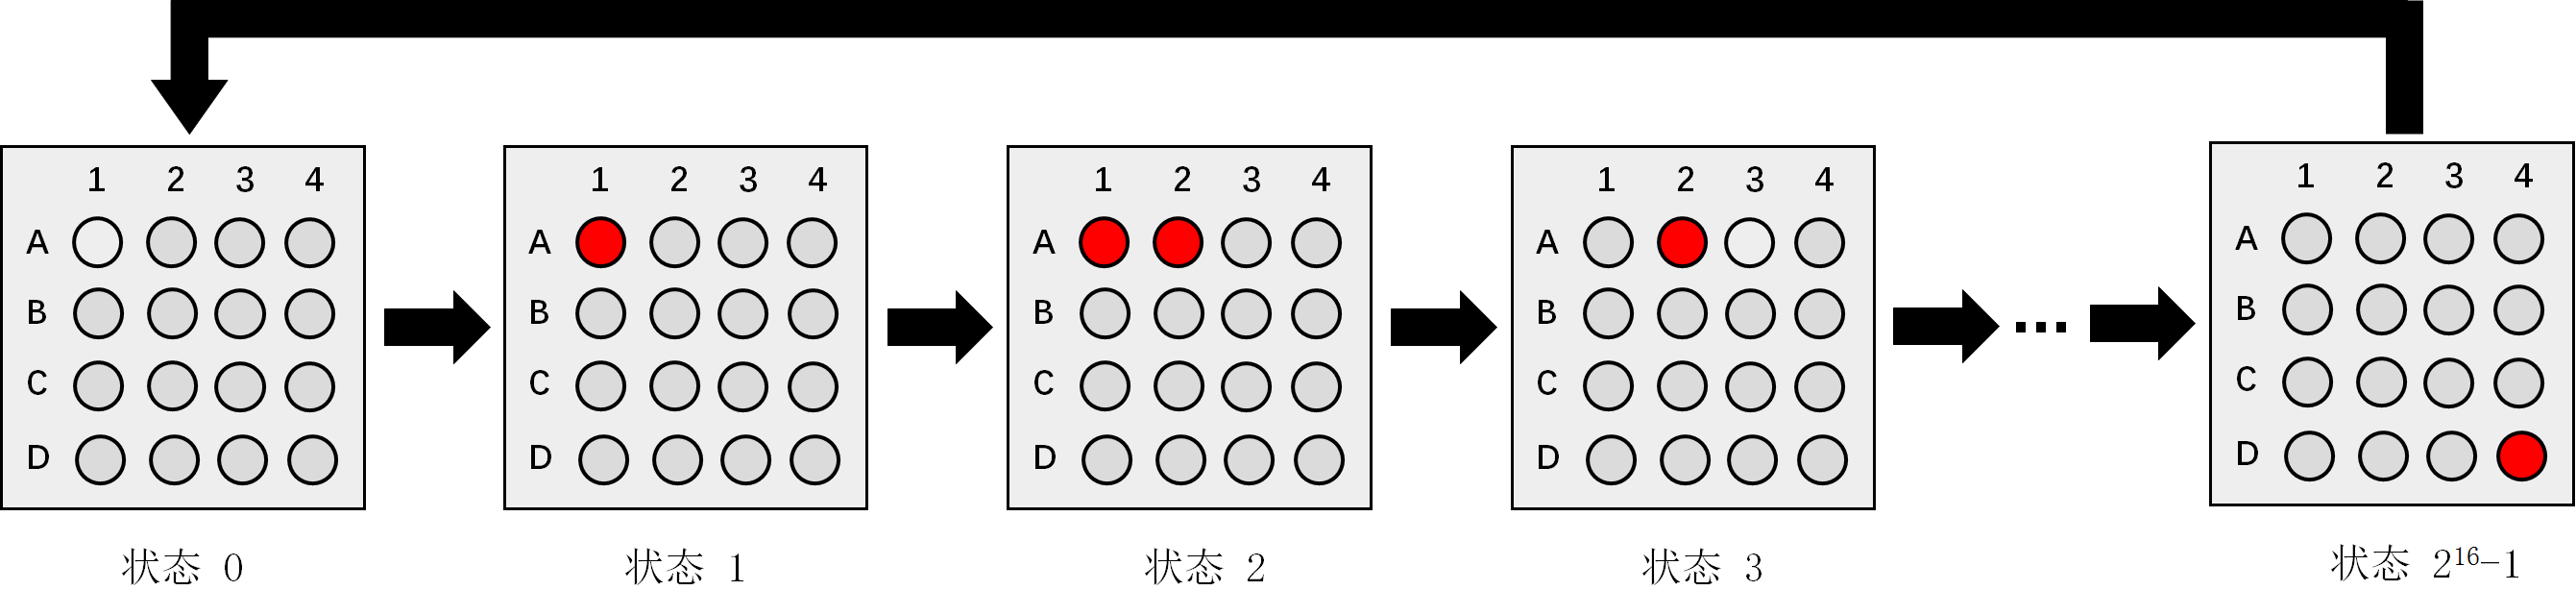
\includegraphics[height=3.6cm, width=14cm]{gray}
  \caption{格雷码编码的点阵状态序列}
  \label{gray}
\end{figure}

使用该编码方法,当LED点阵共包含$n$个LED灯时,一个总的循环周期内共有$2^n$个LED点阵状态,则一个总的循环周期的时间长度为:

\begin{equation}
T = 2^n * t_{dur}
\end{equation}

同二进制编码方法一样,格雷码编码方法也存在状态叠加后的图像不唯一问题。例如状态1、状态2叠加和状态2、状态3叠加后得到的图像相同,无法根据叠加图像识别出正确的拍摄时间。但是,当采用格雷码编码时,如果摄像头曝光时间与控制周期时间相同或小于控制周期时,摄像头将拍摄到一个状态的图像或者是两个状态的叠加图像。根据格雷码特点可知,当一个状态与其相邻状态叠后,只有一位发生变化,因此识别误差相对于二进制编码方法较小。例如,对于4位二进制编码,第3个状态0011与第4个状态0100叠加得到第7个状态0111,与真实状态相差3或4个控制周期。而对于4位格雷码编码,第3个状态0010与第4个状态0110叠加得到第4个状态0110。但是当调整控制周期,使得拍摄图像中有多个状态叠加时,并不能保证只有一位发生变化,仍然会产生较大识别误差。

\subsection{分组叠加编码}

为了解决二进制编码和格雷码编码存在的问题,在格雷码编码的基础上提出分组叠加编码方法。由于在检测过程中拍摄到LED点阵状态叠加是不可避免的,而且状态叠加造成的识别误差是由于叠加状态后得到的码字不唯一所导致,因此可以设计一种编码方式,使得在两种状态叠加时,得到的叠加码字唯一且按规律排列,即使得叠加码字为格雷码。以4位编码为例,状态1、2、3显示的码字分别为0000、0001、0010,则相邻状态叠加得到的叠加码字为0001、0011,满足格雷码编码要求。全部编码序列如图~\ref{over}所示:

\begin{figure}[h] 
  \centering
  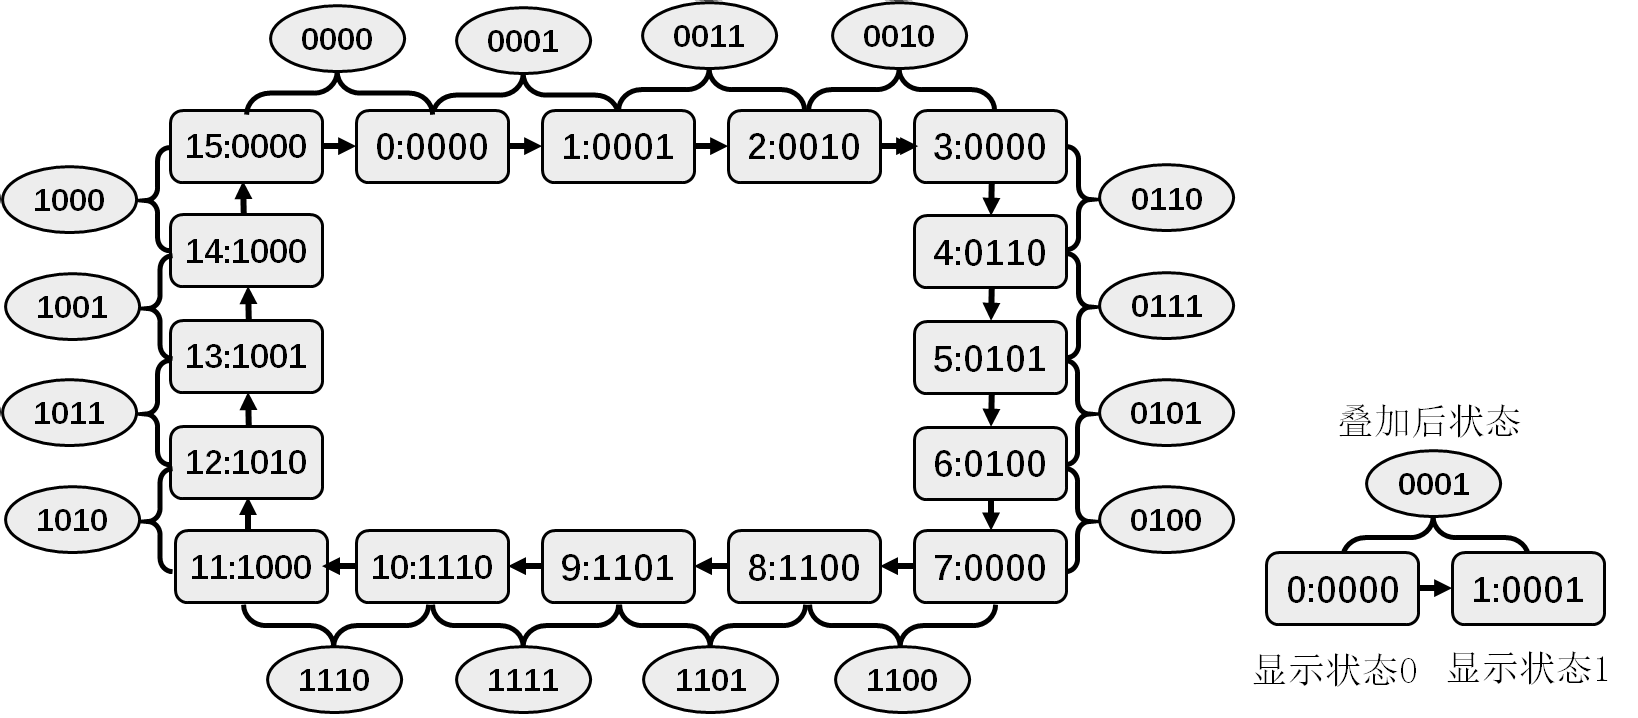
\includegraphics[height=5.5cm, width=14cm]{over}
  \caption{分组叠加编码的码字序列和叠加结果}
  \label{over}
\end{figure}

设定摄像头曝光时间为$k$倍($k$为正整数)控制周期时间长度,则大部分情况下在一个曝光周期内,摄像拍摄到的图像是$k + 1$个LED点阵状态的叠加。仅当曝光开始时间与某一控制周期开始时间相同时,可拍摄到$k$个状态叠加,但此情况出现概率较低。对于一个4 × 4 LED点阵,取$k = 4$,将每行4个LED灯视为一组,共分为4组。每一组分别按照上述编码方法进行编码,显示编号0到15共16个码字。每个码字显示的持续时间为4个控制周期,但是4组LED灯码字分别相差一个控制周期发生变化,这样即可以保证每个控制周期都有一组码字发生变化,又可以保证LED点阵的状态在各个控制周期内不相同。当摄像头对LED点阵进行拍摄时,能够拍摄到$k + 1 = 5$个控制周期的LED点阵状态的叠加图像,此叠加图像内,各组LED灯所显示的码字都发生且仅发生了一次变化,因此4组LED灯的叠加结果分别满足格雷码序列,且拍摄到的叠加图像是唯一的。

当第一组LED灯显示完显示序列内所有16个码字后,如图~\ref{series}所示状态63,为避免与状态0相同进入小循环,使第一组LED灯即将显示的码字序号减1,即显示第14个码字,然后继续按照上述规律进行变化。当第一组LED灯全部循环结束,即显示完状态511后,将第二组显示的码字序号减1继续进行循环。显示序列如图~\ref{series}所示:

\begin{figure}[h] 
  \centering
  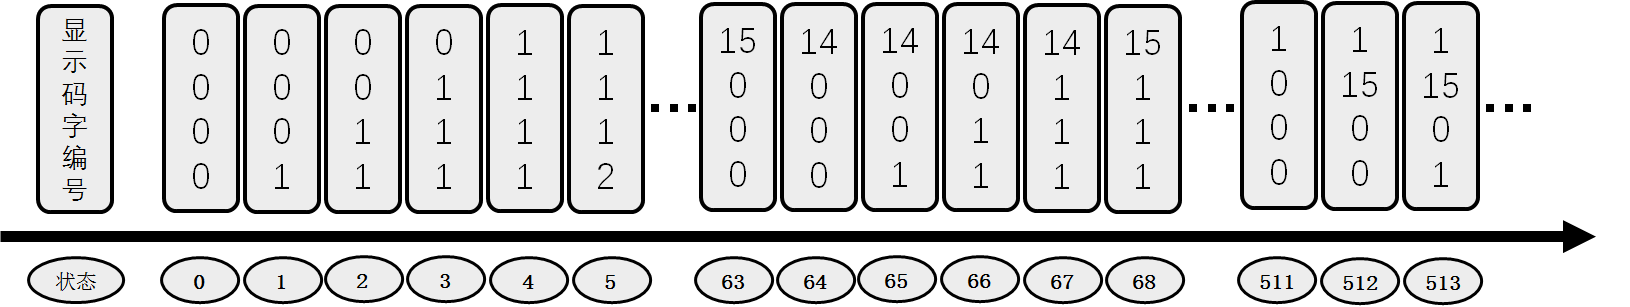
\includegraphics[height=3cm, width=13cm]{series}
  \caption{分组叠加编码的显示序列}
  \label{series}
\end{figure}

具体而言,当摄像头拍摄到状态0至4的叠加图像后,4个组均为第0和第1个码字叠加,因此得到的叠加码字分别为0001、0001、0001、0001。当拍摄到状态1值5时,得到的叠加码字分别为0001、0001、0001、0011。每次拍摄都能得到不同的叠加状态。通过叠加码字可以确定是哪两个显示码字叠加得到,就可以确定摄像头拍摄到的是哪五个状态叠加,从而可以判断摄像头拍摄的开始时刻位于哪个状态内,但是无法判断开始时刻在这个状态内的准确位置。因此检测精度为该状态的持续时间,即控制周期时间长度$t_{dur}$,即曝光时间的四分之一。该编码方法的检测精度($A$)与摄像头曝光时间$t_{exp}$满足如下关系:

\begin{equation}
A = t_{dur} = t_{exp} / k
\end{equation}

则为了提高检测精度,可以降低曝光时间或者增大分组数量。但是一般情况下曝光时间不能过低,因此需要分组数量k较大,也就需要LED点阵中LED灯数量较多。

该方法存在的最大问题在于可操作性欠缺。由于要求各组内相邻两个显示状态叠加而成的叠加状态满足格雷码编码要求,显示状态序列的选取并不存在一定规律。上文示例当中每组包含4个LED灯,而当每组内LED灯数量发生变化时,显示序列同样需要发生变化,且不能保证一定存在满足条件的序列。因此在实际应用当中,该编码方法可操作性较低。

\subsection{进位流水编码}
\label{flowSe}

此方法综合流水编码和分组叠加编码。对于4 × 4 LED点阵,将点阵分为4组,每行1组,每组等级依次升高。每组内各LED灯按照流水编码方法依次点亮。对于等级最低组,即第一组,每个控制周期熄灭当前点亮的LED灯,点亮下一个LED灯。组内最后一个LED灯熄灭后,第一个LED灯点亮,依次循环。对于其他等级组,只有当其低等级组的最后一个LED灯熄灭,发送进位信号给该等级组,该组内才会发生LED灯亮灭变化,熄灭当前点亮的LED灯,点亮下一个LED灯,如图~\ref{composite}所示:

\begin{figure}[h] 
  \centering
  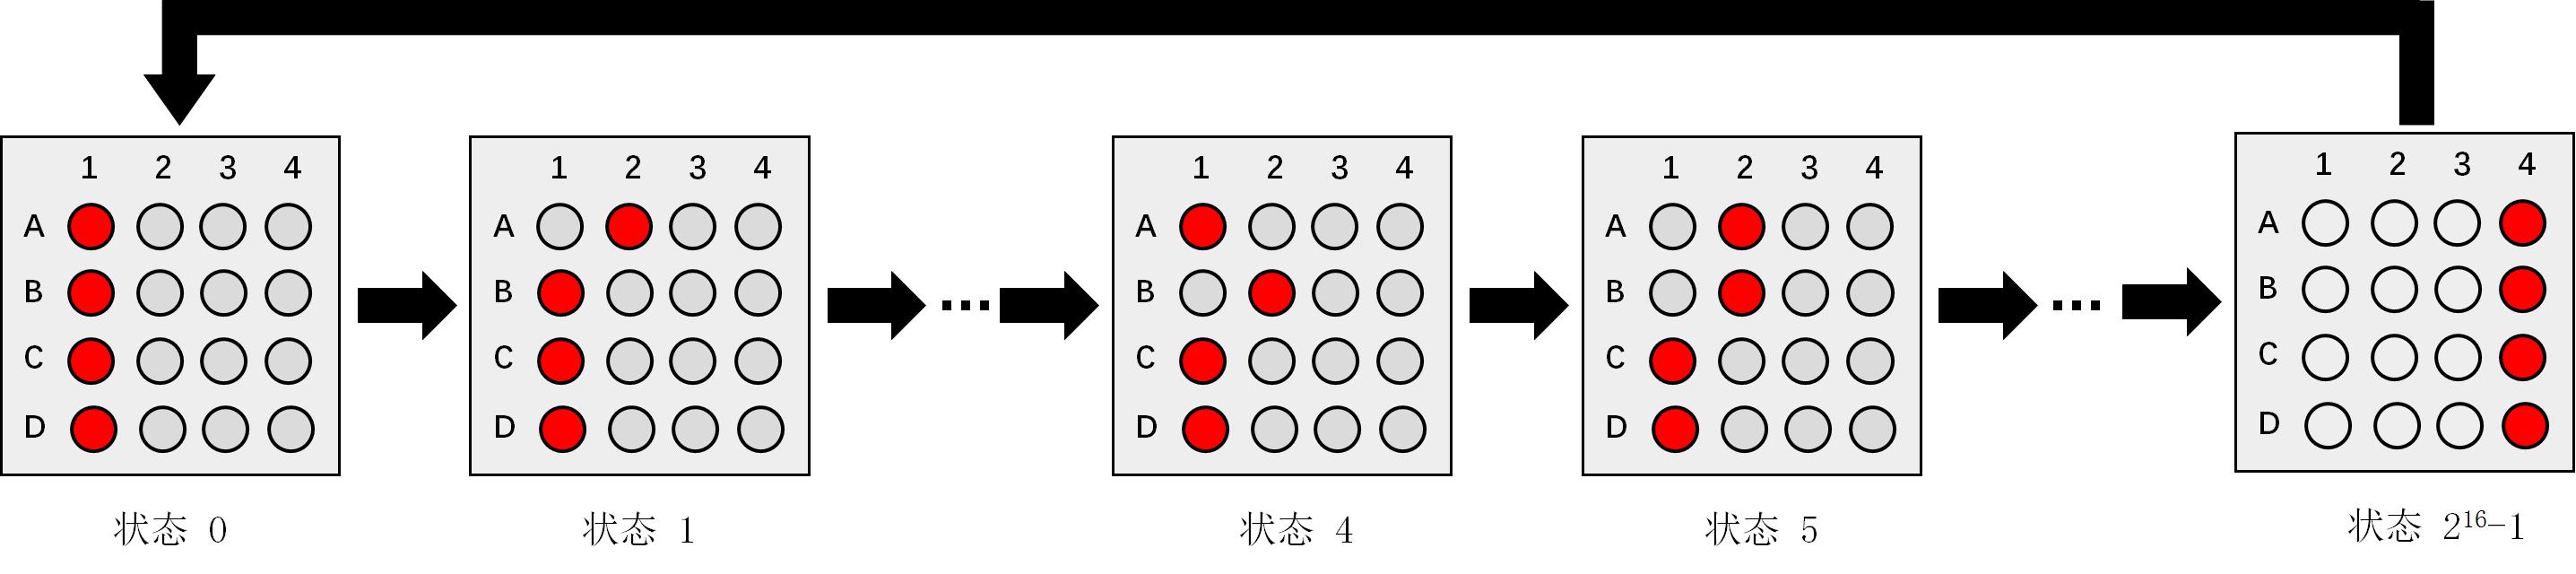
\includegraphics[height=3cm, width=14cm]{composite}
  \caption{进位流水编码的点阵状态序列}
  \label{composite}
\end{figure}

假设控制周期的时间长度为$t_{dur}$,将LED点阵分为k组,每组包含$n_i(i = 0, 1, 2, ..., k-1)$个LED灯,每组内各个LED灯亮灭变化的周期长度为$t_i$。最低等级组的变化周期与控制周期时间相同,即$t_1 = t_{dur}$。因为只有当第一组内所有LED灯循环变化一次后才会向第二组发送进位信号,所以第二等级组的变化周期为$n_1 * t_1$。同理则第$i$组的变化周期为:

\begin{equation}
t_i = t_{dur} * \prod_{j=1}^{i-1} n_j
  \label{4}
\end{equation}

通常情况下,摄像头的曝光时间$t_{exp}$要长于控制周期,因此在摄像头拍摄到的图像内有一个以上的LED灯被点亮。同时,$t_{exp}$要短于最高等级组内所有LED灯变化周期之和$n_k * t_k$,因此在摄像头拍摄到的图像内有一个以上的LED灯是熄灭的。一定可以找到第$i$组,使其满足

\begin{equation}
t_i \le t_{exp} \le n_i * t_i
  \label{5}
\end{equation}

当拍摄到的图像内出现状态叠加时,等级低于$i$的组内所有LED灯均被点亮;第$i$组内部分LED灯被点亮,部分熄灭;等级高于$i$的组内有一个或两个LED灯被点亮。对于等级高于$i$的任一组,当与其相邻的低等级组的最后一个和第一个LED灯被点亮时,说明有进位信号产生,因此该组内有两个灯点亮,否则仅有一个灯点亮。当拍摄到一张满足以上描述的LED点阵图片后,首先找到第一个LED灯非全部点亮的等级组$i$;然后判断第$i$组及等级高于$i$的组内第一个被点亮的LED灯,标记其位置分别为 $P_i, P_i + 1, ..., P_k$。 则摄像头的拍摄时间为:

\begin{equation}
T = \sum_{j=i}^k p_j * t_j
  \label{T}
\end{equation}

根据公式~\ref{T} 可知,拍摄时间的检测精度为第$i$组内各个LED灯的变化周期$t_i$。根据公式~\ref{4} 可知为了提高检测精度,可以减小控制周期和低等级组内LED灯的数量。同时公式~\ref{5} 要求$t_{exp} \le n_i * t_i$,需要同时增加第$i$组内LED灯的数目。因此采用进位流水编码方法进行拍摄时间检测时,可以通过减少控制周期长度和低等级组内LED灯的数量,增加高等级组内LED灯的数量来提高检测精度。

\subsection{编码方法比较}

针对以上5种编码方法,利用包含$n$个LED灯的矩阵,在控制周期为$t_{dur}$,曝光时间为$t_{exp}$的条件下进行比较,比较结果如表~\ref{comp}所示:

\begin{table}[h]
  \centering
  \caption{编码方法比较结果} 
  \label{comp}
  \begin{tabular}{c|c|c|c|c}\hline
  编码方法 & 总循环周期 & 检测精度 & \tabincell{c}{叠加状态\\可识别性}  & \tabincell{c}{摄像头\\参数要求} \\ \hline
  流水编码 & $n * t_{dur}$ & $t_{dur}$ & 是 & 无\\ \hline
  二进制编码 & $2^n * t_{dur}$ & $t_{dur}$ & 否 & 无 \\ \hline
  格雷码编码 & $2^n * t_{dur}$ & $t_{dur}$ & 否 & 有 \\ \hline
  分组叠加编码 & $k * 2 ^ n * t_{dur}$ & $t_{exp} / k$ & 是 & 有 \\ \hline
  进位流水编码 & $2^n * t_{dur}$ & $t_i$ & 是 & 无 \\ \hline
  \end{tabular}
\end{table}

通过比较可以看出,流水编码总循环周期过短,需要检测器包含较多LED灯才能满足检测需求;二进制编码和格雷码编码在状态叠加的情况下存在识别误差,无法准确检测拍摄时间,且需要摄像头曝光时间较短;分组格雷码在进行高精度检测时需要摄像头较短的曝光时间或者检测器包含较多LED灯;进位流水编码克服了以上几种方法存在的问题,能够进行高精度检测。

\section{图像检测算法}
\label{detecSe}

本节主要介绍对于摄像头拍摄到的图像中LED点阵的检测识别算法。当摄像头拍摄到包含LED点阵的图像后,将图片上传给图像处理服务器。服务器首先对图片进行预处理,然后识别各张图片当中LED点阵的位置和各个LED灯的位置、轮廓,并且判断各个LED灯的亮灭状态,再根据LED点阵的编码规律识别LED点阵状态,从而通过状态序列检测摄像头的拍摄时间。

该检测算法主要基于开源计算机视觉库OpenCV(Open Source Computer Vision Library)实现\footnote{http://opencv.org/},采用C++语言实现,部分算法调用OpenCV库函数,完成了对图像数据的处理分析。具体处理过程如下:

\textbf{一、原始数据转换。}由于摄像头在进行拍摄过程当中曝光帧数较多,如果进行拍摄数据压缩需要消耗很大的计算资源,将会引起系统运行延时、中断等不可控问题,因此我们直接获取摄像头拍摄到的原始图像数据,不在本地进行硬件或软件层面的压缩编码。

摄像头拍摄到的原始图像数据为YUV格式,即亮度信息(Y)与色彩信息(UV)分离,采用YUV $4:2:2$格式采样,虽然未经过编码压缩处理,数据量较大,但是在较低帧率条件下摄像头系统能够完成拍摄和保存工作。

为了进一步分析处理图像数据,首先需要对原始图像进行处理,将其转换为较为易于处理的RGB格式,即红(R)、绿(G)、蓝(B)三个颜色通道。这两种格式内的单一通道变量可以用对应的另一种格式内的各个通道的数据表示,两种图像数据格式之间的转换满足如下关系\cite{rumball1992method}:

\begin{equation}
\begin{split}
& \left[
\begin{matrix}
Y \\
U \\
V
\end{matrix}
\right]
=
\left[
\begin{matrix}
0.299 & 0.587 & 0.114 \\
-0.1678 & -0.3313 & 0.5 \\
0.5 & -0.4187 & -0.0813
\end{matrix}
\right]
\left[
\begin{matrix}
R \\
G \\
B
\end{matrix}
\right] \\ \\
& \left[
\begin{matrix}
R \\
G \\
B
\end{matrix}
\right]
=
\left[
\begin{matrix}
1 & 0 & 1.402 \\
1 & -0.34414 & -0.71414 \\
1 & 1.1772 & 0
\end{matrix}
\right]
\left[
\begin{matrix}
Y \\
U \\
V
\end{matrix}
\right]
\end{split}
\label{rgb}
\end{equation}

现阶段对应图像数据的分析处理是在图像处理服务器上完成,服务器性能能够满足运算需求,因此可以采用如上公式进行格式转换。但是在转换过程中需要进行浮点运算,会消耗一部分处理器的运算性能,当后续利用性能较差的摄像头之间进行图像处理时,可以采用其他转换方法进行计算,如查表法、整数转换法等。将图像数据转换后的结果如图~\ref{p1}所示:

\begin{figure}[H] 
  \centering
  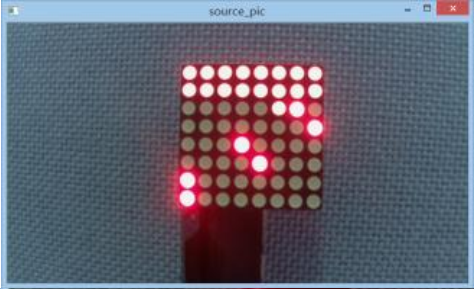
\includegraphics[height=4.5cm, width=7cm]{p1}
  \caption{原始图像}
  \label{p1}
\end{figure}

\textbf{二、灰度图转换。}在得到摄像头拍摄到的RGB图像后,还需要进一步地对图片格式进行转换。对于后期处理来说,RGB图像的三个通道的信息仍存在冗余,因此还需要将其转换为单一通道的灰度图像进行处理。具体的转换过程即利用RGB数据信息,根据公式~\ref{grayG}进行转换,即可利用三通道颜色信息表示图像的灰度信息:

\begin{equation}
Gray = 0.299 * R + 0.587 * G + 0.114 * B
  \label{grayG}
\end{equation}

同样,根据所需精度不同,RGB图像与灰度图像之间的转换可以选取不同的公式。如果不采用浮点运算,且分别采用2位和20位的精度,其转换公式如公式~\ref{gray1},~\ref{gray2}所示。

\begin{align}
& Gray = (1 * R + 2 * G + 1 * B) >> 2
  \label{gray1} \\
& Gray = (313524 * R + 615514 * G + 119538 * B) >> 2
  \label{gray2}
\end{align}

转换为灰度图像如图~\ref{p2}所示。

\begin{figure}[h] 
  \centering
  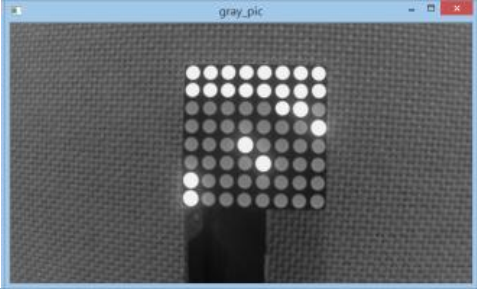
\includegraphics[height=4.5cm, width=7cm]{p2}
  \caption{灰度图像}
  \label{p2}
\end{figure}

\textbf{三、图像模糊处理。}为了减少图像中的噪声和降低图像细节层次,在进一步处理之前需要对图像进行模糊处理。在本章所介绍的算法当中,采用了高斯模糊(Gaussian Blur)来进行处理。

图像模糊的本质利用一种图像滤波器与原图像进行卷积,根据某个像素点在二维图像中其周边各个像素点的取值来估算该点取值。而高斯模糊利用的高斯函数是一种正态分布函数,根据不同的模糊半径可以得到周边各点对于被处理点的贡献权重,二维高斯函数如公式~\ref{Gaussian}所示。

\begin{equation}
G(x,y) = \frac{1}{2 \pi \sigma^2}e^{-(x^2+y^2)/2\sigma ^2}
  \label{Gaussian}
\end{equation}

在具体计算过程中需要将高斯函数转换为矩阵形式,即高斯权重矩阵。通过权重矩阵与原图像像素点矩阵进行卷积,即可得到高斯模糊后的结果。在本算法中,选取5阶权重矩阵,根据二维高斯函数可以计算出权重矩阵如公式~\ref{Gaussian2}所示。

\begin{equation}
K = \frac{1}{159}\left[
\begin{matrix}
2&4&5&4&2 \\
4&9&12&9&4 \\
5&12&15&12&5\\
4&9&12&9&4 \\
2&4&5&4&2 \\
\end{matrix}
\right]
  \label{Gaussian2}
\end{equation}

经过模糊处理后的图像如图~\ref{p3}所示。

\begin{figure}[H] 
  \centering
  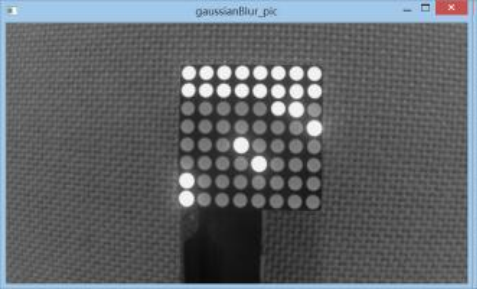
\includegraphics[height=4.5cm, width=7cm]{p3}
  \caption{高斯模糊图像}
  \label{p3}
\end{figure}

\textbf{四、LED灯轮廓提取。}为了提取各个LED灯的边缘轮廓,首先需要坚持图像当中所以的物体边缘。在本算法中采用Canny边缘检测算法 \cite{canny1986computational}。该算法首先利用Sobel算子与图像进行卷积,在二维平面内求解图像当中各个像素点在$X, Y$方向的梯度幅值和方向。然后Canny算法通过设定高低双阈值实现非极大值抑制,找出图像内局部梯度最大值点,即图像边缘点。

然后对于获得的包含边缘的二值图像进行椭圆拟合寻找LED灯轮廓。由于LED灯轮廓均为圆形,且面积相近,可以利用Fitzgibbon等人在文献\cite{fitzgibbon1996buyer}中提出的方法,对二值图像中的边缘进行椭圆拟合,去除掉非椭圆的边缘。同时由于LED灯边缘为圆形,对于长轴和短轴比例超过阈值的拟合椭圆同样予以去除。还有对于面积过大或者过小的非目标椭圆也要去除掉。这样就能够获得所需的LED灯的边缘图像,结果如图~\ref{p4}所示。该步骤所采用的算法均基于OpenCV函数实现,通过调整函数参数可以获得最佳的检测效果。

\begin{figure}[H] 
  \centering
  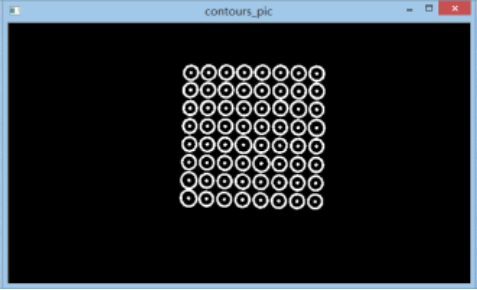
\includegraphics[height=4.5cm, width=7cm]{p4}
  \caption{LED灯边缘图像}
  \label{p4}
\end{figure}

\textbf{五、LED灯状态检测。}根据上一步所检测到的轮廓,可以获得各个LED灯轮廓圆心的所在位置。由于点亮和熄灭的LED灯之间最大的差别在于其亮度的不同,而同为点亮或者熄灭的LED灯之间的亮度差异不大,因此可以根据各个LED灯圆心周围各像素点的亮度值判断LED灯的亮灭状态。具体实现过程中,提取各圆心点所在像素及其周边区域内像素的亮度值,并求取其平均值。然后将所有LED灯的亮度平均值再求平均,则高于次平均值的LED灯即为点亮状态,低于此平均值的LED灯即为熄灭状态。将LED点阵内各个LED灯编号为$L[i][j] (0 \le i, j \le 7)$,其中$i, j$分别表示LED灯所处的行数和列数。检测得到的结果如图~\ref{p5}所示。
 
\begin{figure}[h] 
  \centering
  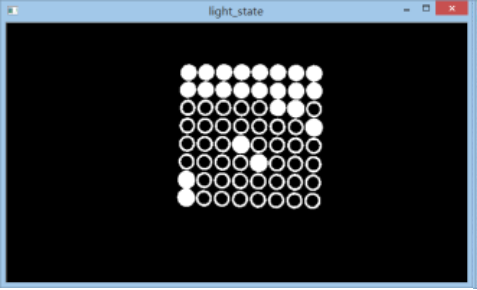
\includegraphics[height=4.5cm, width=7cm]{p5}
  \caption{LED灯状态检测}
  \label{p5}
\end{figure}

\textbf{六、拍摄时间检测。}当得到LED点阵中各个LED灯的亮灭状态后,即可以根据点阵的编码方法计算摄像头拍摄到的点阵状态在序列当中所处的位置,即可以获得摄像头的拍摄时间。如图~\ref{p6}所示,LED点阵按照流水进位方法进行编码,每一行8个LED灯为一组,LED点阵的控制周期$t_{dur}$为0.1ms,根据公式~\ref{4}可知,第二行的LED灯点亮持续时间为$0.1 * 8 = 0.8ms$,第三行为6.4ms。

当摄像头的曝光时间设置为10ms时,第一和第二行LED灯总的点亮时间分别为0.8ms和6.4ms,因此在一个曝光周期内,能够拍摄到第一、二行所有LED灯点亮。而第三行的总点亮时间为51.2ms,长与摄像头曝光周期,因此摄像头拍摄到第三行内两个LED灯点亮。因此可以根据流水进位编码的特点,检测LED点阵内第三到第八行内第一个点亮的LED灯,如图可知分别为$L[2][5], L[3][7], L[4][3], L[5][4], L[6][0], L[7][0]$,因此可以根据公式~\ref{T}计算出摄像头的拍摄时间:

\begin{equation}
\begin{split}
T &= p_3 * t_3 +p_4 * t_4 +p_5 * t_5 +p_6 * t_6 +p_7 * t_7 +p_8 * t_8\\
&=5 \times 6.4 + 7 \times 51.2  +3\times 409.6 + 4\times3276.8  +0\times26214.4  +0\times209715.2\\
&=14726.4 
\end{split}
\end{equation}


\begin{figure}[h] 
  \centering
  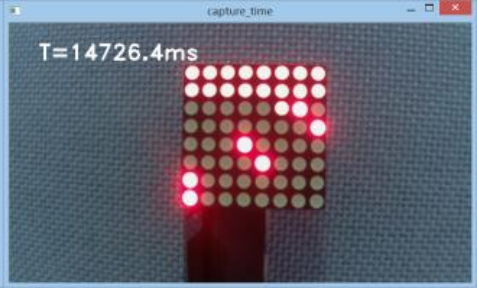
\includegraphics[height=4.5cm, width=7cm]{p6}
  \caption{拍摄时间计算}
  \label{p6}
\end{figure}

\section{本章小结}
本章主要介绍了多摄像头系统拍摄时间的检测方法。该方法主要基于由LED点阵和FPGA组成的检测系统,通过对LED点阵显示的检测信号进行拍摄,并检测拍摄到的点阵状态,从而可以确定各个摄像头的拍摄时间。对于LED点阵检测系统来说,其关键点在于如何构造更加易于识别的点阵状态序列,通过对不同LED点阵编码方法的分析,可以使得摄像头拍摄到的点阵图像能够满足可叠加性和状态序列唯一性,使得摄像头能够在不同的参数设置下识别出点阵状态在序列当中的位置,从而能够更加准确地确定拍摄时间。另外,对于拍摄图像的识别,需要在实际应用过程中,在更加复杂的条件下,更加准确快速地识别出LED点阵的位置,以及各个LED灯亮灭状态,进而计算出拍摄时间。当外界条件发生变化时,可能会对拍摄图像造成印象,影响检测精度,如何克服这个问题,使检测更具有鲁棒性,是下一步研究的重点。



















































